%!TEX root = ../../main.tex
\section{Extraction and treatment of reflection intensity data}
\label{sec:Extraction and treatment of reflection intensity data}

\subsection{Allocating observations to images}
\label{sub:Allocating observations to images}
Before the forward-backward algorithm can be applied, the data for each full observation have to be extracted and allocated to a single diffraction image.
An MTZ file containing the integrated data from the set of diffraction images was produced by processing the images with MOSFLM \cite{leslie2007}.
MTZDUMP, a program from the CCP4 software suite \cite{winn2011}, was used to extract the data from the integrated MTZ file, with additional commands to obtain the space group symmetry and image (batch) information.
A custom script was written to parse the MTZDUMP output and extract the observation information.
Each image is given a \textit{rotation start angle} (RSA) and a \textit{rotation end angle} (REA) and each observation has a \textit{rotation centroid} value.
An observation is allocated to an image if its centroid value lies between the image's RSA and REA.
For fully recorded reflections this is straight forward because the entire observation is recorded on a single image.
This is not the case for partially observed reflections i.e. when a single reflection observation is partially measured on multiple images.
Each detection of a partially measured reflection is given an estimate of the rotation centroid of the full observation.
In theory this centroid value should be the same for each measurement of the same reflection, but in practice this is rarely the case.
To determine the actual centroid value, the mean average of all centroid values of each measurement is calculated, and this value is used to allocate a partial reflection observation to a given image.

At the beginning and end of a data collection experiment, some reflections have not been completely traversed, resulting in observations where the calculated rotation centroid lies outside the oscillation range of the data collection.
In these cases the reflection is allocated to either the first or last image if the calculated centroid is smaller than the RSA of the first image or the REA of the last image respectively.


\subsection{Treatment of intensity data}
\label{sub:Treatment of intensity data}

\subsubsection{Extracting intensity values for fully traversed reflections}
\label{subs:Extracting intensity values for fully traversed reflections}
When reflection observations are integrated with MOSFLM, two intensity estimates are calculated: a profile fitted intensity and a summed intensity.
The profile fitted intensity value is generally a better estimate and this is especially true for weak data.
On the other hand, the summed estimate should be more accurate for the strongest reflections (\url{http://www.ccp4.ac.uk/html/aimless.html}).
In exactly the same manner as utilised in AIMLESS \cite{evans2013}, the custom written parser can use either of the two intensity estimates but defaults to using a combination of the two.
The approach of combining the two is to calculate a weighted average of the two intensity estimates such that the profile fitted estimate is weighted higher for weak reflections and vice versa for strong reflections.
The equation used to extract the combined intensity, $I_{com}$ is
\begin{equation}
    I_{com} = wI_{pr} + (1-w)I_{sum},
\end{equation}
where $I_{pr}$ is the profile fitted intensity estimate, $I_{sum}$ is the summed intensity estimate and $w$ is the weight defined as
\begin{equation}
    w = \f{1}{1 + \left(\f{I_{raw}}{I_{mid}}\right)^{I_{pow}}}.
\end{equation}
In AIMLESS, $I_{pow}$ defaults to 3, $I_{raw}$ is the intensity value before Lorentz-Polarisation (LP) correction and $I_{mid}$ is optimised to give the best overall $R_{meas}$ value.
The custom parser uses $I_{mid} = (I_{pr} + I_{sum})/2$, $I_{raw} = I_{mid} \times $LP and $I_{pow} =$ 3.

The intensity value (either $I_{com}, I_{pr}$ or $I_{sum}$) is calculated for each measurement of a reflection observation.
For full reflections the resulting intensity value is used as the full observation intensity.
For partial reflections this value has to be summed for each measurement of the same reflection observation to obtain the full estimate.

\subsubsection{Estimating the intensity of non-fully traversed reflections}
\label{subs:Estimating the intensity of non-fully traversed reflections}
Some reflection observations are not fully traversed and hence the intensity values for these reflections are incomplete.
Estimates of the true intensity of these reflections can be made by assuming a standard uniform shape for the reflection.
If the reflection is assumed spherical in shape then the measured fraction of the reflection is a spherical cap, shown in Figure~\ref{fig:Spherical Cap}.
\begin{figure}[ht!]
    \centering
    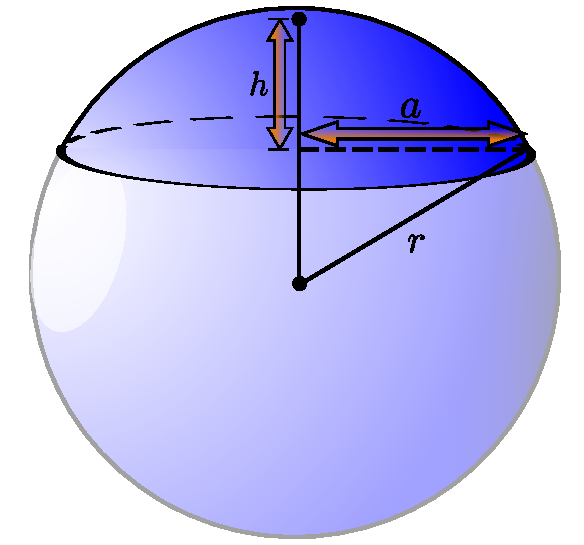
\includegraphics[width=0.6\textwidth]{figures/datared/SphericalCap.pdf}
    \caption[Model of the spherical cap traversed in a data collection experiment.]{Model of the spherical cap traversed in a data collection experiment.
    The translucent volume is the volume that was not recorded.
    $h$ represents the height of the spherical cap, $a$ represents the radius of the circular base of the cap and $r$ is the radius of the sphere.}
    \label{fig:Spherical Cap}
\end{figure}
The ratio of the volume of the spherical cap to the volume of the sphere, $p$ is given by
\begin{equation}
    p = \f{h^2}{d^3} (3d - 2h),
    \label{eq:Spherical cap volume ratio - mine}
\end{equation}
where $d$ is the diameter of the sphere and $h$ is the height of the spherical cap.
If the height of the spherical cap is given as a fraction of the diameter, denoted $q$, and the diameter is set to 1, then equation \ref{eq:Spherical cap volume ratio - mine} becomes
\begin{equation}
    p = 3q^2 - 2q^3,
    \label{eq:eq:Spherical cap volume ratio - Rossman}
\end{equation}
which is the same formula as given in Rossman \textit{et al.} (1979). \nocite{rossmann1979processing}
Angles are used as a proxy for the actual lengths $h$ and $d$ because the lengths are not given.
For reflections where the calculated centroid is before the RSA of the first image, $h$ is approximated as the absolute difference between the RSA of the first image and the mid point of the RSA and REA of the last image on which the reflection was observed.
The spherical diameter of the reflection, $d$ is approximated as twice the absolute difference between the mid point of the RSA and REA of the last image on which the reflection was observed and the rotation centroid.
The analogous values are used for reflections where the reflection centroids were calculated beyond the REA of the last image.

\subsubsection{Quantifying additional uncertainty in the observation variance}
\label{subs:Quantifying additional uncertainty in the observation variance}
The standard deviation for each measurement is also calculated and provided in the output by MOSFLM.
Again, for full reflections this value can be used as the final standard deviation for each measurement.
However, for partial reflections the standard deviations for each partial measurement have to be combined.
This is achieved by summing the variances for each partial measurement giving a total variance denoted $\sigma^2_{sum}$.

However, two more factors complicate the variance calculation.
Firstly, it is acknowledged that the crystal is in a slightly different dose state at each image: hence in combining the variances it is also necessary to increase the uncertainty due to the change in crystal state between images.
This additive uncertainty factor is calculated as
\begin{equation}
    \sigma_{im}^2 = \sum_i^{\text{images}} (1 - (\bs{D}^{im}_i)^2) I^{im}_i,
\end{equation}
where the sum is over all images on which the measurements of an observation are recorded, $I^{im}_i$ is the measured intensity of the observation a image $i$ and $\bs{D}^{im}_i$ is defined as
\begin{equation}
    \bs{D}^{im}_i = \exp(-2 |\Delta B_{i}^{diff}|\sin^2(\theta) / \lambda^2)),
\end{equation}
where $\Delta B_{i}^{diff}$ is the difference in B factor between image $i$ and the centroid image.

Secondly, the total fraction of each measurement is calculated for each reflection (denoted \verb+FRACTIONCALC+ in the MTZ column from MOSFLM).
The sum of these values for partial measurements of an individual observation should be equal to 1.
This is rarely the case because these values are not accurate.
In AIMLESS the criteria for an observation to be regarded as fully recorded over its partial measurements is if the sum of the \verb+FRACTIONCALC+ is bewteen 0.95 and 1.05.
The criterion used by the custom parser script only flags observations where the sum is less than 0.95.
If this is the case then the observations can either be rejected, or the variance of the intensity value can be further inflated by a value proportional to the inverse of the total calculated fraction.
Explicitly the additive factor is calculated as
\begin{equation}
    \sigma^2_{fr} = \varepsilon \times \Sigma \times (1-fr_{tot}),
\end{equation}
where $\varepsilon$ is multiplicity of the reflection, $\Sigma$ is the expected intensity value and $fr_{tot}$ is the sum of the individual calculated fractions for each partial measurement.

The final variance for a single observation is then given by
\begin{equation}
    \sigma^2 = \sigma^2_{sum} + \sigma_{im}^2 + \sigma^2_{fr}.
\end{equation}
